% Fixed-position renderer for Figure 3: Level 2 DFD for 0.1 User Authentication
% and Access Control. Keep labels and directed flows synchronized with f.1.mmd.
\documentclass{article}
\usepackage[paperwidth=14cm,paperheight=19cm,margin=0cm]{geometry}
\usepackage{tikz}
\usetikzlibrary{arrows.meta,calc}
\pagestyle{empty}
\setlength{\parindent}{0pt}

\definecolor{processfill}{HTML}{E0E7FF}
\definecolor{processstroke}{HTML}{4338CA}
\definecolor{entityfill}{HTML}{F3F4F6}
\definecolor{entitystroke}{HTML}{374151}
\definecolor{flowstroke}{HTML}{8A8A80}

\tikzset{
  process/.style={
    circle, draw=processstroke, fill=processfill, line width=0.8pt,
    minimum size=3.15cm, text width=2.65cm, align=center, inner sep=1pt,
    font=\sffamily\small
  },
  entity/.style={
    rectangle, draw=entitystroke, fill=entityfill, line width=0.7pt,
    minimum width=3.0cm, minimum height=0.78cm, align=center, inner sep=2pt,
    font=\sffamily\small
  },
  datastore/.style={
    minimum width=5.2cm, minimum height=1.15cm,
    align=center, inner sep=2pt, font=\sffamily\small
  },
  datastoreline/.style={draw=entitystroke,line width=0.85pt},
  flow/.style={
    -{Stealth[length=1.9mm,width=1.3mm]}, draw=flowstroke, line width=0.6pt,
    rounded corners=3pt
  },
  flowlabel/.style={
    fill=white, fill opacity=0.88, text opacity=1, inner sep=1.3pt,
    align=center, font=\sffamily\scriptsize
  }
}

\begin{document}
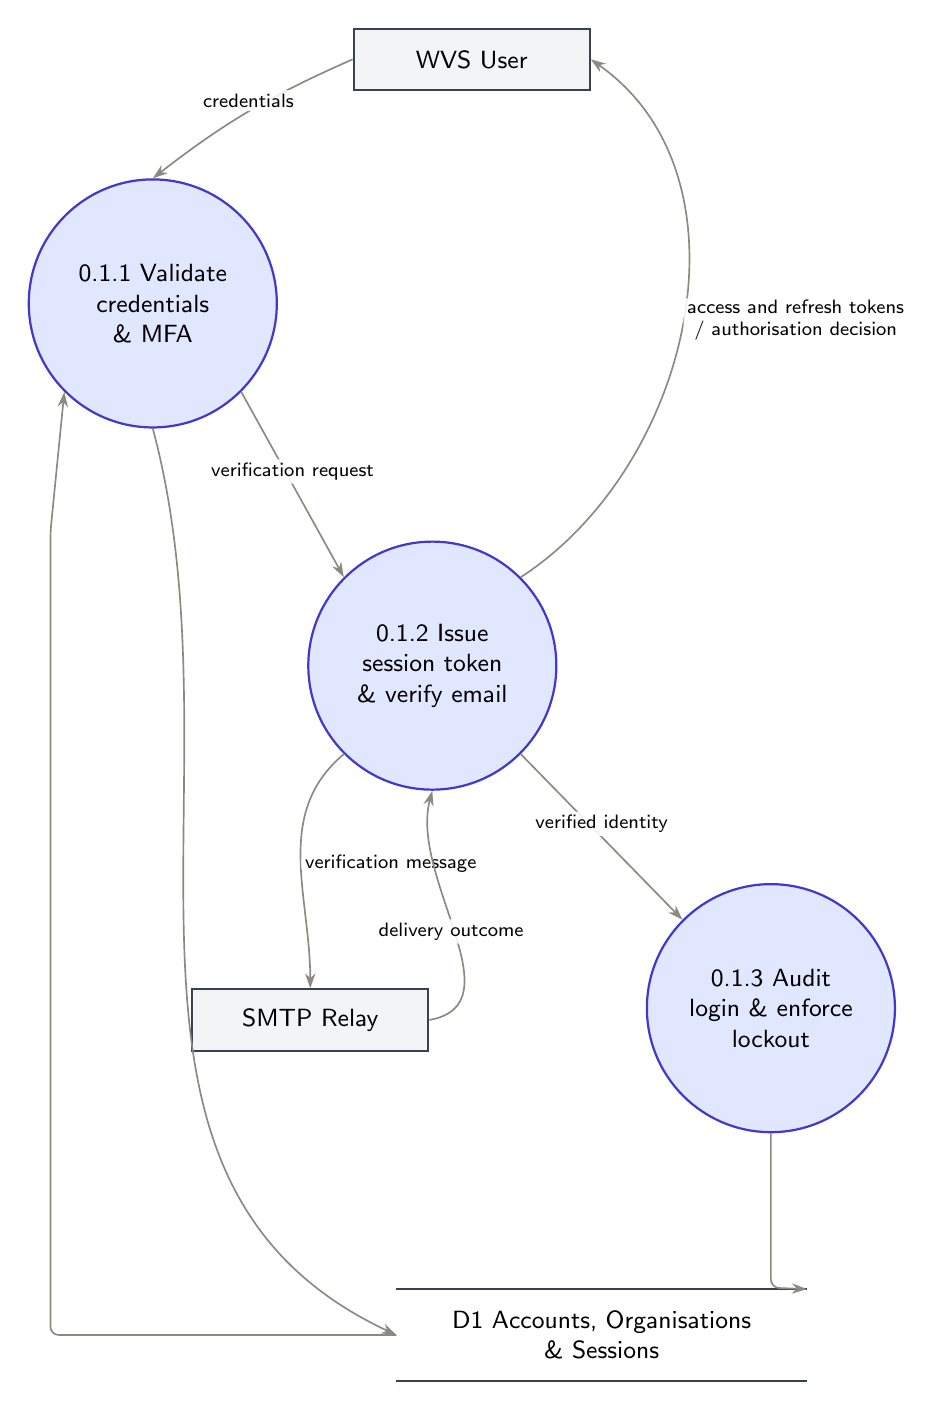
\begin{tikzpicture}[x=1cm,y=1cm]
  \node[entity] (user) at (6.90,17.75) {WVS User};
  \node[process] (p11) at (2.85,14.65) {0.1.1 Validate credentials\\\& MFA};
  \node[process] (p12) at (6.40,10.05) {0.1.2 Issue session token \\\& verify email};
  \node[process] (p13) at (10.70,5.70) {0.1.3 Audit login \& enforce\\lockout};
  \node[entity] (smtp) at (4.85,5.55) {SMTP Relay};
  \node[datastore] (d1) at (8.55,1.55) {D1 Accounts, Organisations\\\& Sessions};
  \draw[datastoreline] (d1.north west) -- (d1.north east);
  \draw[datastoreline] (d1.south west) -- (d1.south east);

  % User authentication and session workflow.
  \draw[flow] (user.west) to[bend right=7]
    node[flowlabel,above] {credentials} (p11.north);
  \draw[flow] (p11.south east) -- node[flowlabel,above] {verification request} (p12.north west);
  \draw[flow] (p12.north east) to[out=33,in=-35]
    node[flowlabel,right,pos=0.50] {access and refresh tokens\\/ authorisation decision} (user.east);
  \draw[flow] (p12.south east) -- node[flowlabel,above] {verified identity} (p13.north west);

  % Account-store interactions; use separate outer lanes to keep directions legible.
  \draw[flow] (d1.west) -- (1.55,1.55) -- (1.55,11.75) -- (p11.south west);
  \draw[flow] (p11.south) to[out=-75,in=155] (d1.west);
  \draw[flow] (p13.south) -- (10.70,2.15) -- (d1.north east);

  % Email verification exchange.
  \draw[flow] (p12.south west) to[out=220,in=90]
    node[flowlabel,right,pos=0.52] {verification message} (smtp.north);
  \draw[flow] (smtp.east) to[out=10,in=-105]
    node[flowlabel,below,pos=0.55] {delivery outcome} (p12.south);
\end{tikzpicture}
\end{document}
